\documentclass[12pt]{article}

\usepackage{graphicx}
\usepackage{algorithm}
\usepackage{float}
\usepackage{algpseudocode}

\title{COSC 528: Project 3}
\author{Ian Lumsden}

\begin{document}
	\pagenumbering{gobble}
	\maketitle
	\newpage
	\pagenumbering{arabic}
	
	\section{Objective}
	The goal of this project was to classify breast tumors as malignant or benign using the provided data. In the first part of the project, a k-nearest-neighbors algorithm was implemented and used to classify the data. In the second part, a decision tree algorithm was implemented using \textit{entropy}, \textit{Gini Index}, and \textit{misclassification error} as the possible impurity measures. The decision tree was also used to classify the data. Then, the hyperparameters of both models were optimized using cross-validation. Finally, the dimensionality of the data was reduced using Principal Component Analysis (PCA), and the decision tree was applied to this reduced data. 
	
	\section{Preprocessing}
	The provided data was contained in the "breast-cancer-wisconsin.data" file. It consists of 691 rows of the following 11 unlabeled features:
	\begin{enumerate}
		\item \textbf{Sample Code Number}: ID Number
		\item \textbf{Clump Thickness}: Discrete from 1-10
		\item \textbf{Uniformity of Cell Size}: Discrete from 1-10
		\item \textbf{Uniformity of Cell Shape}:
		Discrete from 1-10
		\item \textbf{Marginal Adhesion}: Discrete from 1-10
		\item \textbf{Single Epithelial Cell Size}: Discrete from 1-10
		\item \textbf{Bare Nuclei}: Discrete from 1-10
		\item \textbf{Bland Chromatin}: Discrete from 1-10
		\item \textbf{Normal Nucleoli}: Discrete from 1-10
		\item \textbf{Mitoses}: Discrete from 1-10
		\item \textbf{Class}: Discrete (2 for benign, 4 for malignant)
	\end{enumerate}
    \paragraph{}
    The first feature (Sample Code Number) was dropped as it provided no meaningful data to the classification. Additionally, there were several NaN values in the Bare Nuclei column. These were removed by replacing them with the mean of the other elements in the feature column. Then, the class labels were adjusted so that 2 became 0 and 4 became 1. Finally, roughly 30 percent of the dataset was not unique. Initially, all this data was included in the dataset. However, after all models were implemented and tested, it was determined that the models were slightly more accurate when all but the first instance of non-unique data was removed. Therefore, all the results listed are based on the fully unique dataset.
    
    \section{K-Nearest-Neighbors}
    The first algorithm for this project was k-nearest-neighbors. It is a classification algorithm that, unlike other algorithms, primarily uses logic to perform classification. This algorithm's "training" stage consists only of storing the training instances and labels. During classification, distances between the data element to be classified and each training element are calculated. Then, the \textit{k} closest training elements are used to poll for the class of the new data.
    \paragraph{}
    The specific implementation of k-nearest-neighbors used for this project was mostly the same as the generic description. The distance measure used in this implementation was Euclidean distance, which is defined below:
    \begin{equation}
        \label{Eq:1}
    	d_i = \sqrt{\sum_{f=0}^{8} (y_f - x_f)^2} = ||\mathbf{y} - \mathbf{x}||,
    \end{equation}
    where \textbf{y} is the data to be classified, \textbf{x} is the current training element, and $f$ represents the features. The one primary difference between this project's implementation and the generic implementation was that the polling for the classification was weighted using the inverse of the distance. The polling score for a class was defined by
    \begin{equation}
    	\label{Eq:2}
    	s^i = \sum_{d \in \delta^i} \frac{1}{d},
    \end{equation}
    where $s^i$ represents the score for class $i$ and $\delta^i$ is the subset of the calculated distances in which the training element used was of class $i$. The algorithm used is described by the pseudo-code in algorithm 1.
    \begin{algorithm} \label{kNN}
    	\caption{k-Nearest-Neighbors Pseudo-Code}
    	\begin{algorithmic}
    		\State $train\_data \Leftarrow$ Passed Training Data
    		\State $train\_labels \Leftarrow$ Passed Training Labels
    		\State $cdata \Leftarrow$ Array of Data to be Classified
    		\State $clabels \Leftarrow$ []
    		\For {elem in cdata}
    		\State $distances \Leftarrow$ []
    		\For {train\_elem in train\_data}
    		\State Append result of $euclidean\_distance(elem, train\_elem)$ to distances
    		\EndFor
    		\State Sort distances
    		\State $ks \Leftarrow$ first k elements of distances
    		\State $s0 \Leftarrow$ 0
    		\State $s1 \Leftarrow$ 0
    		\For {dist in ks}
    		\If {training element corresponding to dist is class 0}
    		\State $s0 = s0 + \frac{1}{dist}$
    		\Else
    		\State $s1 = s1 + \frac{1}{dist}$
    		\EndIf
    		\EndFor
    		\If {$s0 > s1$}
    		\State Add 0 to $clabels$ as class for $elem$
    		\Else
    		\State Add 1 to $clabels$ as class for $elem$
    		\EndIf
    		\EndFor
    		\State Return $clabels$
    	\end{algorithmic} 
    \end{algorithm}
    \paragraph{}
    Once the k-nearest-neighbors algorithm was implemented, cross-validation was used to determine the best value of $k$ for the dataset. The following result statistics were calculated to determine the best value:
    \begin{enumerate}
    	\item \textbf{Number of True Negatives (TN)}
    	\item \textbf{Number of False Negatives (FN)}
    	\item \textbf{Number of True Positives (TP)}
    	\item \textbf{Number of False Positives (FP)}
    	\item \textbf{Confusion Matrix}: Set of TN, FN, TP, and FP
    	\item \textbf{Accuracy}: $\frac{TN + TP}{TN + TP + FN + FP}$
    	\item \textbf{True Positive Rate (TPR)}: $\frac{TP}{TP + FN}$
    	\item \textbf{Positive Predictive Value (PPV)}: $\frac{TP}{TP + FP}$
    	\item \textbf{True Negative Rate (TNR)}: $\frac{TN}{TN + FP}$
    	\item \textbf{$F_1$ Score}: $\frac{2* PPV * TPR}{PPV + TPR}$ 
    \end{enumerate}
    The statistics can be found in Appendix A. Based on the statistics, the k-nearest-neighbors algorithm performed the best with $k \ge 3$. Since the algorithm is naturally faster at lower values of $k$, the best $k$ value for this dataset is 3.
    \section{Decision Tree}
    For the second part of the project, a decision tree algorithm was used to classify the dataset. The training for the decision tree algorithm consists of creating a tree in which the nodes are features and the traversal is controlled by inequalities applied to the features. The root node of each subtree is determined by finding the feature with the lowest impurity measure.
    \paragraph{}
    The decision tree implementation for this project was implemented so that it could use one of three different impurity measures: \textit{entropy}, \textit{Gini Index}, and \textit{misclassification error}. For binary classification, the equation for \textit{entropy} is
    \begin{equation}
        \label{Eq.3}
    	\phi(p) = -p\log_{2}(p) - (1-p)\log_{2}(1-p),
    \end{equation}
    where $p$ is the probability of class 0. The equation for \textit{Gini Index} is
    \begin{equation}
    	\label{Eq.4}
    	\phi(p) = 2p(1-p),
    \end{equation}
    and the equation for \textit{misclassification error} is
    \begin{equation}
    	\label{Eq.5}
    	\phi(p) = 1 - \max(p, 1-p).
    \end{equation}
    \paragraph{}
    The implementation used for this project allows for the impurity measure, maximum tree depth, and impurity threshold to be set prior to training. During training, it constructs a binary decision tree where decision rules are less-than and greater-than-or-equal-to inequalities about the same splitting value. Data is classified by traversing the decision tree. The pseudo-code for the implementation for training is in algorithm 2.
     \begin{algorithm} \label{DT}
    	\caption{Decision Tree Pseudo-Code}
    	\begin{algorithmic}
    		\Procedure{getBestSplit}{$feature$}
    		\State $best\_impurity \Leftarrow$ 2
    		\State $best\_split \Leftarrow$ -1
    		\For {splitPoint in range(min, max, 0.5)}
    		\State $p \Leftarrow \frac{Number of Class 0 in Split 1}{Number of Elements in Split 1}$
    		\State $q \Leftarrow \frac{Number of Class 0 in Split 2}{Number of Elements in Split 2}$
    		\State $imp1 \Leftarrow$ Impurity from $p$
    		\State $imp2 \Leftarrow$ Impurity from $q$
    		\If {$imp1 + imp2 < best\_impurity$}
    		\State $best\_impurity \Leftarrow imp1 + imp2$
    		\State $best\_split \Leftarrow splitPoint$
    		\EndIf
    		\EndFor
    		\State Return best\_impurity and best\_split
    		\EndProcedure
    		
    		
    		\Procedure{addNode}{$data$}
    		\State $splits \Leftarrow$ []
    		\For {f in features}
    		\State Append $getBestSplit(f)$ to splits
    		\EndFor
    		\State Sort splits by impurity
    		\If {splits[0] can have non-leaf children (based on max depth and impurity threshold)}
    		\State Add splits[0] to tree
    		\State $addNode($data[data < splitPoint]$)$
    		\State $addNode($data[data $\ge$ splitPoint$)$
    		\Else
    		\State Add splits[0] to tree
    		\State Add leaf (most probable class in split 1) as left child
    		\State Add leaf (most probable class in split 2) as right child
    		\EndIf
       		\EndProcedure
    		
    		\Procedure{train}{$train\_data$, $train\_labels$}
    		\State $tdata \Leftarrow$ merge train\_data and train\_labels	
    		\State $addNode(tdata)$
    		\EndProcedure
    	\end{algorithmic} 
    \end{algorithm}
    \paragraph{}
    After implementing the model, cross-validation was performed using the same statistics as for  k-nearest-neighbors. For decision trees, these statistics were calculated for all combinations of impurity measures, maximum depths, and impurity thresholds. All statistics are not listed due to the amount of data. After analyzing the statistics, it was determined that the following three combinations produce the best results (all are the same):
    \begin{enumerate}
    	\item Gini Index with maximum depth of 6 or 7 and impurity threshold of 0.0
    	\item Entropy with maximum depth of 6 or 7 and impurity threshold of 0.0, 0.1, or 0.2
    	\item Misclassification Error with maximum depth of 6 or 7 and impurity threshold of 0.0
    \end{enumerate}
    Table \ref{dtstats} lists the statistics for all of these combinations.
    \begin{table}[]
    	\centering
    	\begin{tabular}{|c | c|}
    		\hline
    		Statistics & Values\\ \hline
    	    True Negative & 113 \\
    	    False Negative & 7 \\
    	    True Positive & 54 \\
    	    False Positive & 1 \\
    	    Accuracy & 0.9542857142857143 \\
    	    True Positive Rate & 0.8852459016393442 \\
    	    Positive Predictive Value & 0.9818181818181818 \\
    	    True Negative Rate & 0.9912280701754386 \\
    	    $F_1$ Score & 0.9310344827586207 \\ \hline
        \end{tabular}
        \caption{Best Statistics for Decision Trees}\label{dtstats}
    \end{table}

    \section{Principal Component Analysis (PCA)}
    To try to improve the decision tree algorithm, Principal Component Analysis was applied to the data.
    \paragraph{}
    To begin, the preprocessed data, $X$, was factored using singular value decomposition (SVD). This process converts the data into the following
    \begin{equation}
    X = U \Sigma V^T,
    \end{equation}
    where $U$ is an $m x m$ unitary matrix, $\Sigma$ is a diagonal $m x n$ matrix of eigenvalues, and $V$ is a $n x n$ unitary matrix of eigenvectors. The diagonal values of $\Sigma^2$ represent the variance that each principal component covers. By dividing by the sum of variances, the percentage of variance that each primary component covers was obtained. These percentages were plotted against the number of the principal component, as shown in Figs. \ref{ScreeTrain} and \ref{ScreeTest}. There are two graphs because the data was already split between training and testing sets, so the PCA was performed on each set individually.
    \begin{center}
        \begin{figure}[H]
    	    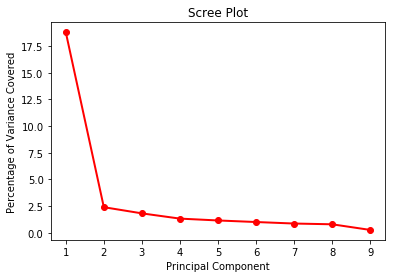
\includegraphics[width=0.75\linewidth]{Pictures/screeTrain.png}
    	    \caption{Scree Graph for SVD on the Training Set}
    	    \label{ScreeTrain}
        \end{figure}
    \end{center}
    \begin{center}
        \begin{figure}[H]
    	    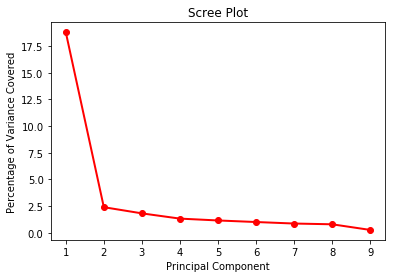
\includegraphics[width=0.75\linewidth]{Pictures/screeTest.png}
    	    \caption{Scree Graph for SVD on the Testing Set}
    	    \label{ScreeTest}
        \end{figure}
    \end{center}
    From Figs. \ref{ScreeTrain} and \ref{ScreeTest}, the first primary component clearly covered the most of the data's variance. However, none of the other features were clearly more important than the others. For visual purposes, the PCA was first performed to produce a two-dimensional reduced dataset. The equations for PCA are as follows
    \begin{equation}
    W = XV^\prime = U^\prime S^\prime,
    \end{equation}
    where X is the initial dataset, the prime symbol indicates that a matrix has been reduced to its first $k$ columns, and W is the final reduced dataset.
    \paragraph{} 
    After implementing this equation using numpy, a graph (Figs. \ref{PCATrain} and \ref{PCATest}) was made of the two principal components, with one on each axis. 
    \begin{center}
        \begin{figure}[H]
    	    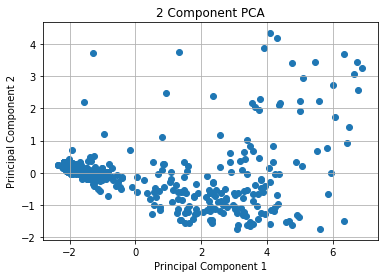
\includegraphics[width=0.75\linewidth]{Pictures/pcatrain.png}
        	\caption{Relationship between the two primary components in the training data}
    	    \label{PCATrain}
        \end{figure}
    \end{center}
    \begin{center}
    	\begin{figure}[H]
    		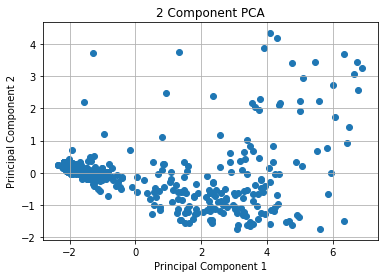
\includegraphics[width=0.75\linewidth]{Pictures/pcatest.png}
    		\caption{Relationship between the two primary components in the testing data}
    		\label{PCATest}
    	\end{figure}
    \end{center}
    \paragraph{}
    Finally, the decision tree cross-validation is repeated for PCA data obtained from values of $k$ (number of reduced dimensions) between 2 and 9, inclusive. After analyzing the statistics, all values of $k$ produced the same statistics: one set for \textit{Gini Impurity} and \textit{entropy} and another for \textit{misclassification error}. The first set of statistics is in Table \ref{gestats}, and the second set is in Table \ref{mestats}.
    \begin{table}[H]
    	\centering
    	\begin{tabular}{|c | c|}
    		\hline
    		Statistics & Values\\ \hline
    		True Negative & 84 \\
    		False Negative & 38 \\
    		True Positive & 23 \\
    		False Positive & 30 \\
    		Accuracy & 0.6114285714285714 \\
    		True Positive Rate & 0.3770491803278688 \\
    		Positive Predictive Value & 0.4339622641509434 \\
    		True Negative Rate & 0.7368421052631579 \\
    		$F_1$ Score & 0.40350877192982454 \\ \hline
    	\end{tabular}
    	\caption{Statistics for \textit{Gini  Index} and \textit{Entropy} for PCA data}\label{gestats}
    \end{table}
    \begin{table}[H]
    	\centering
    	\begin{tabular}{|c | c|}
    		\hline
    		Statistics & Values\\ \hline
    		True Negative & 88 \\
    		False Negative & 40 \\
    		True Positive & 21 \\
    		False Positive & 26 \\
    		Accuracy & 0.6228571428571429 \\
    		True Positive Rate & 0.3442622950819672 \\
    		Positive Predictive Value & 0.44680851063829785 \\
    		True Negative Rate & 0.7719298245614035 \\
    		$F_1$ Score & 0.38888888888888884 \\ \hline
    	\end{tabular}
    	\caption{Statistics for \textit{Misclassification Error} for PCA data}\label{mestats}
    \end{table}

    \section{Conclusions}
    From the data above, both k-nearest-neighbors and decision trees are shown to be good classifiers for potentially cancerous breast tumors. Although both produce very similar results, this implementation of k-nearest-neighbors appears to be slightly more accurate than this implementation of a decision tree classifier. Both models could probably be improved if there were more unique elements in the dataset. For k-nearest-neighbors, the model could also possibly be improved by using a different distance measure, such as Mahalanobis or Chi Square distance. The decision tree model could probably be improved by using a different tree structure, such as a B-Tree. However, the high accuracy of the decision tree model on the unmodified data combined with the low accuracy of the model on the PCA data suggests that there is an issue in the PCA algorithm. The issue likely stems from either the normalizing of the data prior to applying PCA or the linear algebra used in implementing the PCA. However, given the high accuracy of the two models, a fully-functioning PCA would likely not produce significantly better results than the models on the raw data. As a result, applying PCA would likely not be needed. 
    
    \section{Code}
    The following is a breakdown of the code files for this project:
    \begin{itemize}
    	\item \textbf{driver.ipynb}: a Jupyter Notebook that is used as the "main" program
    	\item \textbf{kNN.py}: the implementation of k-nearest-neighbors (as a class) and the model's supporting functions
    	\item \textbf{decision\_tree.py}: the implementation of the decision tree model (as a pair of classes) and the model's supporting functions
    	\item \textbf{PCA.py}: the implementation of PCA and its supporting and visualization functions
    \end{itemize}
    
    \newpage
    \section{Appendix A}
    \begin{enumerate}
    	\item $k = 2$
    	\begin{itemize}
    		\item True Negative: 112
    		\item False Negative: 4
    		\item True Positive: 57
    		\item False Positive: 2
    		\item Accuracy: 0.9657142857142857
    		\item True Positive Rate: 0.9344262295081968
    		\item Positive Predictive Value: 0.9661016949152542
    		\item True Negative Rate: 0.9824561403508771
    		\item $F_1$ Score: 0.95
    	\end{itemize}
        \item $k = 3$
        \begin{itemize}
        	\item True Negative: 112
        	\item False Negative: 3
        	\item True Positive: 58
        	\item False Positive: 2
        	\item Accuracy: 0.9714285714285714
        	\item True Positive Rate: 0.9508196721311475
        	\item Positive Predictive Value: 0.9666666666666667
        	\item True Negative Rate: 0.9824561403508771
        	\item $F_1$ Score: 0.9586776859504132
        \end{itemize}
        \item $k = 4$
        \begin{itemize}
        	\item True Negative: 112
        	\item False Negative: 3
        	\item True Positive: 58
        	\item False Positive: 2
        	\item Accuracy: 0.9714285714285714
        	\item True Positive Rate: 0.9508196721311475
        	\item Positive Predictive Value: 0.9666666666666667
        	\item True Negative Rate: 0.9824561403508771
        	\item $F_1$ Score: 0.9586776859504132
        \end{itemize}
        \item $k = 5$
        \begin{itemize}
        	\item True Negative: 112
        	\item False Negative: 3
        	\item True Positive: 58
        	\item False Positive: 2
        	\item Accuracy: 0.9714285714285714
        	\item True Positive Rate: 0.9508196721311475
        	\item Positive Predictive Value: 0.9666666666666667
        	\item True Negative Rate: 0.9824561403508771
        	\item $F_1$ Score: 0.9586776859504132
        \end{itemize}
        \item $k = 6$
        \begin{itemize}
        	\item True Negative: 112
        	\item False Negative: 3
        	\item True Positive: 58
        	\item False Positive: 2
        	\item Accuracy: 0.9714285714285714
        	\item True Positive Rate: 0.9508196721311475
        	\item Positive Predictive Value: 0.9666666666666667
        	\item True Negative Rate: 0.9824561403508771
        	\item $F_1$ Score: 0.9586776859504132
        \end{itemize}
        \item $k = 7$
        \begin{itemize}
        	\item True Negative: 112
        	\item False Negative: 3
        	\item True Positive: 58
        	\item False Positive: 2
        	\item Accuracy: 0.9714285714285714
        	\item True Positive Rate: 0.9508196721311475
        	\item Positive Predictive Value: 0.9666666666666667
        	\item True Negative Rate: 0.9824561403508771
        	\item $F_1$ Score: 0.9586776859504132
        \end{itemize}
        \item $k = 8$
        \begin{itemize}
        	\item True Negative: 112
        	\item False Negative: 3
        	\item True Positive: 58
        	\item False Positive: 2
        	\item Accuracy: 0.9714285714285714
        	\item True Positive Rate: 0.9508196721311475
        	\item Positive Predictive Value: 0.9666666666666667
        	\item True Negative Rate: 0.9824561403508771
        	\item $F_1$ Score: 0.9586776859504132
        \end{itemize}
        \item $k = 17$
        \begin{itemize}
        	\item True Negative: 112
        	\item False Negative: 3
        	\item True Positive: 58
        	\item False Positive: 2
        	\item Accuracy: 0.9714285714285714
        	\item True Positive Rate: 0.9508196721311475
        	\item Positive Predictive Value: 0.9666666666666667
        	\item True Negative Rate: 0.9824561403508771
        	\item $F_1$ Score: 0.9586776859504132
        \end{itemize}
        \item $k = 33$
        \begin{itemize}
        	\item True Negative: 112
        	\item False Negative: 3
        	\item True Positive: 58
        	\item False Positive: 2
        	\item Accuracy: 0.9714285714285714
        	\item True Positive Rate: 0.9508196721311475
        	\item Positive Predictive Value: 0.9666666666666667
        	\item True Negative Rate: 0.9824561403508771
        	\item $F_1$ Score: 0.9586776859504132
        \end{itemize}
    \end{enumerate}
	
\end{document}